\section{Representing a roadmap as a graph}
\label{sec:l13-graphs}
A graph $G=(V,E)$ consists of vertices (nodes) and edges connecting them.
It can represent a road network, communication links, or any specified
relationship. In a roadmap, intersections are nodes and the individual
paths joining adjacent intersections are edges. Start, goal, and their
projections are also inserted as nodes; a projection inside a branch splits
that branch into two edges.

An undirected edge permits travel in both directions. Directed edges
represent allowed directions separately. A simple computer representation
stores node identifiers and edge records $(u,v,w)$, where $w$ is the cost
of traversing the edge. Neighbor lists provide another convenient
representation. The graph drawing is a visualization of these records;
its layout need not preserve physical distances. To execute a route, retain
the geometric path associated with each edge as well.

\begin{figure}[htbp]
\centering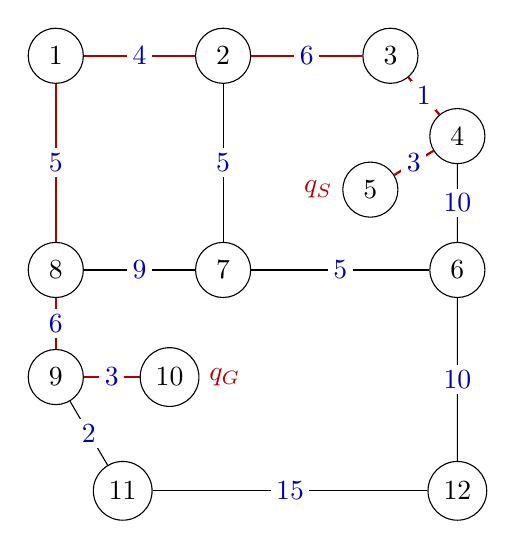
\begin{tikzpicture}[scale=.85,n/.style={circle,draw,fill=white,minimum size=7mm},w/.style={fill=white,inner sep=2pt,text=blue!70!black}]
\foreach \i/\x/\y in {1/0/5,2/2.5/5,3/5/5,4/6/3.8,5/4.7/3,6/6/1.8,7/2.5/1.8,8/0/1.8,9/0/.2,10/1.7/.2,11/1/-1.5,12/6/-1.5}
 \node[n] (n\i) at (\x,\y) {$\i$};
\foreach \a/\b/\c in {1/2/4,1/8/5,2/3/6,2/7/5,3/4/1,4/5/3,4/6/10,6/7/5,6/12/10,7/8/9,8/9/6,9/10/3,9/11/2,11/12/15}
 \draw (n\a)--(n\b) node[midway,w] {$\c$};
\foreach \a/\b in {5/4,4/3,3/2,2/1,1/8,8/9,9/10}
 \draw[red!70!black,thick] (n\a)--(n\b);
\foreach \a/\b/\c in {5/4/3,4/3/1,3/2/6,2/1/4,1/8/5,8/9/6,9/10/3}
 \path (n\a)--(n\b) node[midway,w] {$\c$};
\node[left,red!70!black] at (n5.west) {$q_S$};
\node[right,red!70!black] at (n10.east) {$q_G$};
\end{tikzpicture}

\caption{An undirected weighted roadmap graph. Node 5 is the start and
node 10 is the goal; nodes 4 and 9 represent their roadmap projections.
Weights are assigned example costs, not measurements of this drawing.
The red edges show the minimum-cost route.}
\label{fig:l13-weighted}
\end{figure}

For a sequence of adjacent nodes $v_0,\ldots,v_m$, the path cost is
\begin{equation}
 J=\sum_{k=0}^{m-1}w(v_k,v_{k+1}).
 \label{eq:l13-pathcost}
\end{equation}
If weights are physical lengths, minimizing $J$ finds a shortest route
on the graph. Other choices can represent time or penalties. A graph
route is not necessarily the shortest path in the continuous free space.
For the assigned weights in Figure~\ref{fig:l13-weighted}, the visually
plausible route $5,4,6,7,8,9,10$ costs
$3+10+5+9+6+3=36$. A systematic search finds a route of cost 28.

\section{Dijkstra's algorithm}
\label{sec:l13-dijkstra}
Dijkstra's algorithm applies to nonnegative edge costs. It maintains a
best known cumulative cost $g(v)$ from the start and a predecessor $p(v)$
for each reached node. An \emph{open} node has a tentative cost and awaits
selection. A \emph{settled} node has been selected with minimum open cost;
its cost is then final.

\subsection{Selection and relaxation}
\begin{enumerate}
\item Set $g(q_S)=0$ and all other costs to infinity. Put the start in
the open set; initially there are no predecessors or settled nodes.
\item Select the node $u$ with smallest $g(u)$ among \emph{all} open
nodes. Remove it from the open set and settle it.
\item If $u=q_G$, stop successfully. Otherwise consider each unsettled
neighbor $v$ and form the candidate $g(u)+w(u,v)$.
\item If this candidate is smaller than $g(v)$, replace $g(v)$ and set
$p(v)=u$. Insert $v$ into the open set or update its priority there.
This operation is called \emph{relaxation}.
\item Repeat. If the open set becomes empty before the goal is selected,
there is no route from start to goal in this graph.
\end{enumerate}
The selection is global over the frontier, not restricted to neighbors
of the most recently expanded node. Nonnegative weights ensure that an
alternative path through a node with higher tentative cost cannot later
improve the node just settled. Zero-weight edges are allowed; equal-cost
choices can be resolved consistently without changing the optimal cost.

\subsection{A complete trace}
For the graph in Figure~\ref{fig:l13-weighted}, the selection order and
successful updates are:
\begin{center}
\begin{tabular}{crl}
\toprule
Selected node & Final cost & New or improved tentative costs\\
\midrule
5 & 0 & $g(4)=3$\\
4 & 3 & $g(3)=4,\quad g(6)=13$\\
3 & 4 & $g(2)=10$\\
2 & 10 & $g(1)=14,\quad g(7)=15$\\
6 & 13 & $g(12)=23$; candidate 18 for node 7 rejected\\
1 & 14 & $g(8)=19$\\
7 & 15 & No improvement: candidate 24 for node 8 rejected\\
8 & 19 & $g(9)=25$\\
12 & 23 & $g(11)=38$\\
9 & 25 & $g(10)=28,\quad g(11):38\to27$\\
11 & 27 & No improvement\\
10 & 28 & Goal selected: stop\\
\bottomrule
\end{tabular}
\end{center}
Node 11 illustrates a predecessor change: it is initially reached from
12 at cost 38, then improved through 9 to cost 27. Node 12 must be selected
before 9 because $23<25$, even though the drawing places node 9 nearer
the goal. Dijkstra uses accumulated cost rather than visual direction.

\begin{figure}[htbp]
\centering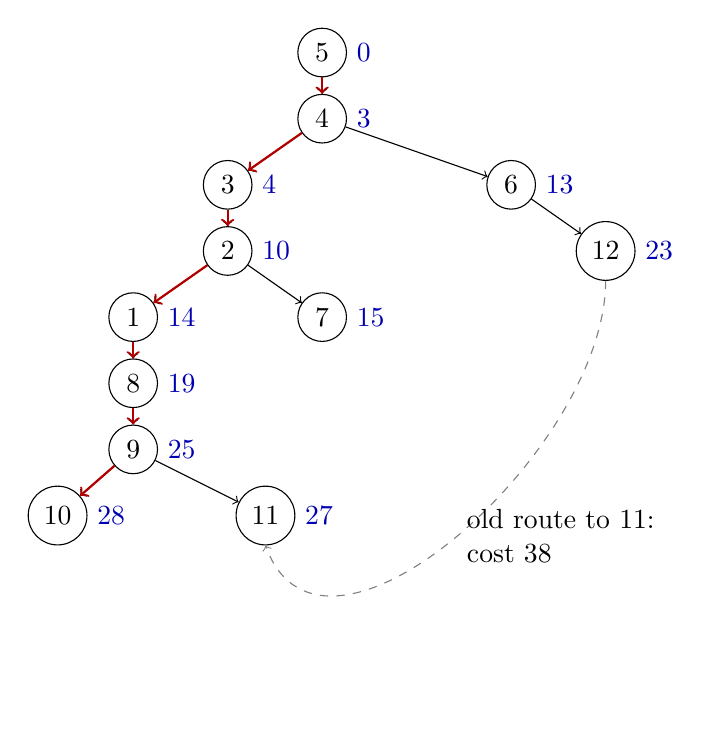
\begin{tikzpicture}[x=1.2cm,y=.6cm,n/.style={circle,draw,fill=white,minimum size=6mm}]
\foreach \i/\x/\y/\g in {5/0/0/0,4/0/-1.4/3,3/-1/-2.8/4,6/2/-2.8/13,2/-1/-4.2/10,1/-2/-5.6/14,7/0/-5.6/15,8/-2/-7/19,9/-2/-8.4/25,10/-2.8/-9.8/28,11/-.6/-9.8/27,12/3/-4.2/23} {
\node[n] (n\i) at (\x,\y) {$\i$};
\node[right,blue!70!black] at (n\i.east) {$\g$};}
\foreach \a/\b in {5/4,4/3,4/6,3/2,2/1,2/7,1/8,8/9,9/10,9/11,6/12}
 \draw[->] (n\a)--(n\b);
\foreach \a/\b in {5/4,4/3,3/2,2/1,1/8,8/9,9/10}
 \draw[->,red!70!black,thick] (n\a)--(n\b);
\draw[->,dashed,gray] (n12) to[out=-90,in=-70] node[right,align=left,text=black] {old route to 11:\\cost 38} (n11.south);
\end{tikzpicture}

\caption{Predecessor tree at termination, with cumulative costs in blue.
The dashed link is the superseded predecessor of node 11, first reached
through 12 at cost 38. The final red chain reconstructs the solution.
Only one final predecessor is retained for each non-root node.}
\label{fig:l13-tree}
\end{figure}

During a hand execution one may draw duplicate candidate occurrences of
a graph node and cross out the more expensive ones. In a cost/predecessor
implementation these occurrences correspond to comparisons against the
same stored $g(v)$. A better candidate changes that node's predecessor;
it does not create a distinct physical location.

Once the goal is selected, follow predecessors backward:
\[
 10\leftarrow9\leftarrow8\leftarrow1\leftarrow2\leftarrow3
 \leftarrow4\leftarrow5.
\]
Reverse this list to obtain the forward route. Its cost is
\[
 3+1+6+4+5+6+3=28.
\]
Each consecutive pair identifies an original roadmap edge. Executing the
route follows those stored geometric curves, rather than new straight
segments between node positions.

\subsection{Why discovering the goal is not enough}
Node 10 is first discovered at cost 28 while node 11 remains open at 27.
The algorithm must select 11 before declaring 10 optimal. In the original
graph this produces no further improvement, but the rule is essential.

To see why, modify the graph by replacing $w(9,11)=2$ with 1 and adding
an undirected edge $(11,10)$ of weight 1. Node 9 now discovers node 10 at
28 and improves node 11 to 26. Expanding 11 improves the goal to
$26+1=27$, giving
\[
 5\to4\to3\to2\to1\to8\to9\to11\to10.
\]
Stopping at first discovery would return the inferior cost 28. The correct
stopping event is selecting the goal as the minimum-cost open node.

\section{A brief introduction to A*}
A* prioritizes an open node by
\begin{equation}
 f(v)=g(v)+h(v),
 \label{eq:l13-astar}
\end{equation}
where $h(v)$ estimates the remaining cost to the goal. This can concentrate
the search on promising regions and reduce the number of expanded nodes.
Setting $h=0$ recovers Dijkstra's selection rule. The heuristic changes
the exploration order, not the definition of the accumulated path cost.

When nodes have Cartesian positions and edge weights are lengths of
physical paths, straight-line distance to the goal is a useful heuristic.
It does not overestimate the remaining route length. It also satisfies
the consistency condition $h(u)\le w(u,v)+h(v)$ for every edge, so an
A* graph search that settles nodes need not reopen them. With a merely
admissible but inconsistent heuristic, improved nodes may need reopening
to retain optimality.

Arbitrary example weights do not automatically support an unscaled
Cartesian-distance heuristic. Its units and lower-bound property must
match the chosen cost. A* does not permanently discard a branch merely
because it initially points away from the goal; obstacles can require
such detours. A useful heuristic can save work, but faster execution is
not guaranteed for every problem.

\section{Exact cell decomposition by a sweep line}
\label{sec:l13-sweep}
Another way to construct a planning graph is to partition the free region
into simple cells. For polygonal obstacles and a polygonal outer boundary,
choose a fixed sweep direction. At each vertex event, introduce parallel
cuts through free space. A full-cut construction extends each event line
through every free interval of the domain; it can subdivide more than
the minimal vertical decomposition, but remains an exact decomposition.
Obstacle interiors are excluded from the cells.

Between consecutive event coordinates the boundaries are straight and
do not change order. Each connected free cell is a triangle or trapezoid
(including rectangular cases) and is convex. Convexity means the segment
between any two points in the cell stays in the cell. A nonconvex region
does not have this property for every pair of points.

\begin{figure}[htbp]
\centering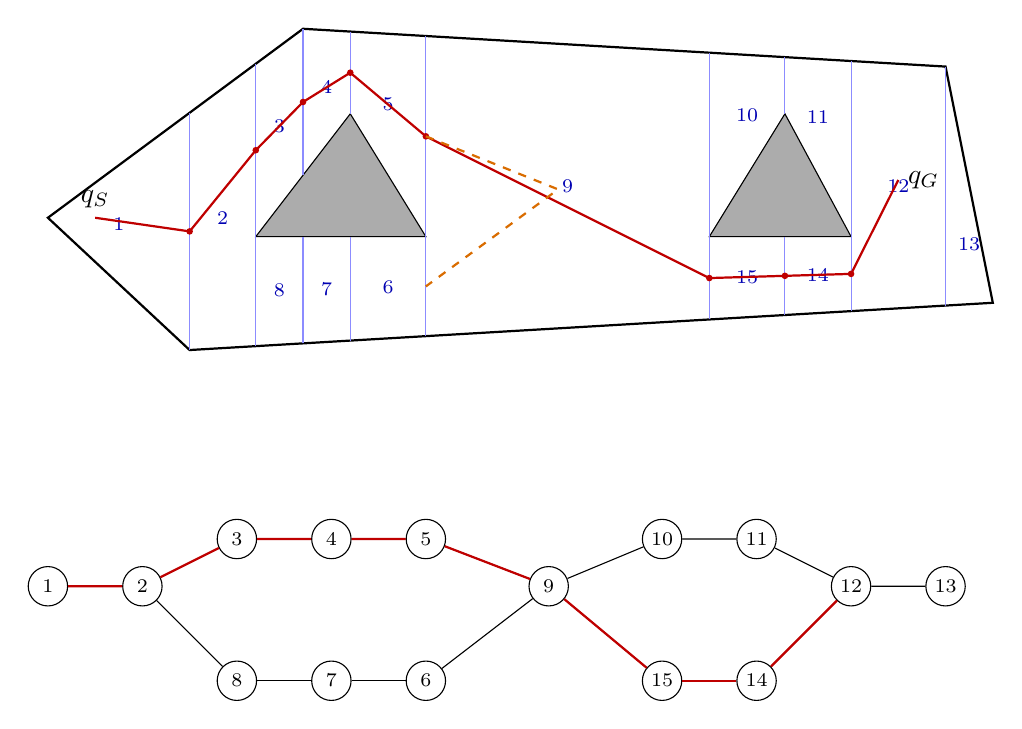
\begin{tikzpicture}[scale=1.2]
\draw[thick] (0.0000,1.4000)--(2.7000,3.4000)--(9.5000,3.0000)--(10.0000,0.5000)--(1.5000,0.0000)--cycle;
\filldraw[fill=gray!65] (2.2000,1.2000)--(3.2000,2.5000)--(4.0000,1.2000)--cycle;
\filldraw[fill=gray!65] (7.0000,1.2000)--(7.8000,2.5000)--(8.5000,1.2000)--cycle;
\draw[thin,blue!45] (1.5000,0.0000)--(1.5000,2.5111);
\draw[thin,blue!45] (2.2000,0.0412)--(2.2000,1.2000);
\draw[thin,blue!45] (2.2000,1.2000)--(2.2000,3.0296);
\draw[thin,blue!45] (2.7000,0.0706)--(2.7000,1.2000);
\draw[thin,blue!45] (2.7000,1.8500)--(2.7000,3.4000);
\draw[thin,blue!45] (3.2000,0.1000)--(3.2000,1.2000);
\draw[thin,blue!45] (3.2000,2.5000)--(3.2000,3.3706);
\draw[thin,blue!45] (4.0000,0.1471)--(4.0000,1.2000);
\draw[thin,blue!45] (4.0000,1.2000)--(4.0000,3.3235);
\draw[thin,blue!45] (7.0000,0.3235)--(7.0000,1.2000);
\draw[thin,blue!45] (7.0000,1.2000)--(7.0000,3.1471);
\draw[thin,blue!45] (7.8000,0.3706)--(7.8000,1.2000);
\draw[thin,blue!45] (7.8000,2.5000)--(7.8000,3.1000);
\draw[thin,blue!45] (8.5000,0.4118)--(8.5000,1.2000);
\draw[thin,blue!45] (8.5000,1.2000)--(8.5000,3.0588);
\draw[thin,blue!45] (9.5000,0.4706)--(9.5000,3.0000);
\node[blue!70!black,font=\scriptsize] at (0.7500,1.3278) {1};
\node[blue!70!black,font=\scriptsize] at (1.8500,1.3955) {2};
\node[blue!70!black,font=\scriptsize] at (2.4500,0.6279) {8};
\node[blue!70!black,font=\scriptsize] at (2.4500,2.3699) {3};
\node[blue!70!black,font=\scriptsize] at (2.9500,0.6426) {7};
\node[blue!70!black,font=\scriptsize] at (2.9500,2.7801) {4};
\node[blue!70!black,font=\scriptsize] at (3.6000,0.6618) {6};
\node[blue!70!black,font=\scriptsize] at (3.6000,2.5985) {5};
\node[blue!70!black,font=\scriptsize] at (5.5000,1.7353) {9};
\node[blue!70!black,font=\scriptsize] at (7.4000,0.7735) {15};
\node[blue!70!black,font=\scriptsize] at (7.4000,2.4868) {10};
\node[blue!70!black,font=\scriptsize] at (8.1500,0.7956) {14};
\node[blue!70!black,font=\scriptsize] at (8.1500,2.4647) {11};
\node[blue!70!black,font=\scriptsize] at (9.0000,1.7353) {12};
\node[blue!70!black,font=\scriptsize] at (9.7500,1.1176) {13};
\draw[red!75!black,thick] (0.5000,1.4000)--(1.5000,1.2556)--(2.2000,2.1148)--(2.7000,2.6250)--(3.2000,2.9353)--(4.0000,2.2618)--(7.0000,0.7618)--(7.8000,0.7853)--(8.5000,0.8059)--(9.0000,1.8000);
\fill[red!75!black] (1.5000,1.2556) circle(.035);
\fill[red!75!black] (2.2000,2.1148) circle(.035);
\fill[red!75!black] (2.7000,2.6250) circle(.035);
\fill[red!75!black] (3.2000,2.9353) circle(.035);
\fill[red!75!black] (4.0000,2.2618) circle(.035);
\fill[red!75!black] (7.0000,0.7618) circle(.035);
\fill[red!75!black] (7.8000,0.7853) circle(.035);
\fill[red!75!black] (8.5000,0.8059) circle(.035);
\node[above] at (0.5000,1.4000) {$q_S$};
\node[right] at (9.0000,1.8000) {$q_G$};
\draw[orange!85!black,thick,dashed] (4.0000,2.2618)--(5.4,1.7)--(4.0000,0.6735);
\begin{scope}[yshift=-3.5cm,n/.style={circle,draw,fill=white,minimum size=5mm,inner sep=1pt,font=\scriptsize}]
\node[n] (n1) at (0.0000,1.0000) {1};
\node[n] (n2) at (1.0000,1.0000) {2};
\node[n] (n3) at (2.0000,1.5000) {3};
\node[n] (n4) at (3.0000,1.5000) {4};
\node[n] (n5) at (4.0000,1.5000) {5};
\node[n] (n9) at (5.3000,1.0000) {9};
\node[n] (n10) at (6.5000,1.5000) {10};
\node[n] (n11) at (7.5000,1.5000) {11};
\node[n] (n12) at (8.5000,1.0000) {12};
\node[n] (n13) at (9.5000,1.0000) {13};
\node[n] (n8) at (2.0000,0.0000) {8};
\node[n] (n7) at (3.0000,0.0000) {7};
\node[n] (n6) at (4.0000,0.0000) {6};
\node[n] (n15) at (6.5000,0.0000) {15};
\node[n] (n14) at (7.5000,0.0000) {14};
\draw (n1)--(n2);
\draw (n2)--(n3);
\draw (n2)--(n8);
\draw (n3)--(n4);
\draw (n4)--(n5);
\draw (n8)--(n7);
\draw (n7)--(n6);
\draw (n5)--(n9);
\draw (n6)--(n9);
\draw (n9)--(n10);
\draw (n10)--(n11);
\draw (n11)--(n12);
\draw (n9)--(n15);
\draw (n15)--(n14);
\draw (n14)--(n12);
\draw (n12)--(n13);
\draw[red!75!black,thick] (n1)--(n2);
\draw[red!75!black,thick] (n2)--(n3);
\draw[red!75!black,thick] (n3)--(n4);
\draw[red!75!black,thick] (n4)--(n5);
\draw[red!75!black,thick] (n5)--(n9);
\draw[red!75!black,thick] (n9)--(n15);
\draw[red!75!black,thick] (n15)--(n14);
\draw[red!75!black,thick] (n14)--(n12);
\end{scope}
\end{tikzpicture}

\caption{Full vertical cuts through polygon vertices partition the free
region into 15 convex cells. The connectivity graph records free portals
between cells. The red route uses the sequence
$1,2,3,4,5,9,15,14,12$; the orange detour illustrates passing through an
interior point when entering and leaving cell 9 on the same side.
The geometry preserves the two-obstacle layout and cell numbering.}
\label{fig:l13-cells}
\end{figure}

\subsection{Connectivity and geometric reconstruction}
Represent each cell by a graph node. Connect cells that share a
traversable boundary interval, called a \emph{portal}. Mere contact at
an obstacle vertex does not create a usable passage when obstacle contact
counts as collision. Identify the cells containing $q_S$ and $q_G$, then
search their connectivity graph.

The result is initially a sequence of cells, not yet a geometric path.
Choose a point in the relative interior of each free portal, such as its
midpoint. Connect the start, successive portal points, and the goal with
segments inside the corresponding cells. Convexity keeps those segments
inside cell closures, but obstacle boundaries are forbidden. If two portal
points lie on the same supporting line and their direct connection runs
along an obstacle, insert a point strictly inside the cell and connect
through it instead. This occurs for the sequence $5,9,6$ in the figure.

The complete procedure is therefore:
\begin{enumerate}
\item Decompose the free region with parallel sweep cuts.
\item Number the cells and construct the portal-adjacency graph.
\item Locate the start and goal cells and run graph search.
\item Select free portal points along the returned sequence.
\item Construct and check the geometric segments, adding interior
waypoints where necessary.
\end{enumerate}
An unweighted adjacency graph can minimize the number of cell transitions.
That objective is not necessarily geometric path length. To optimize a
length cost, the graph representation and weights must account for the
actual connectors being used. Similarly, exact decomposition describes
the represented geometry faithfully; it does not imply exact knowledge
of a real environment or automatic dynamic feasibility of the path.
